\section{Design of the Delay and \gls{reverb} Effect}
In this section, the delay and the \gls{reverb} will be designed to fit intro a \gls{dsp}, which mean that a discreet block diagram is obtained and afterwords the equation to the implementation is made. Afterwords the assembly code is developed and implemented. 


\subsection{Obtaining the Differential Equation}
The Delay and \gls{reverb} effect are very similar in their design so they will be presented and designed in the same section. The block diagram presented in \autoref{} is changed so it fit intro a \gls{iir} filter construction. The \gls{iir} filter is chosen because the \gls{fir} filter will require lots more power. To get a naturally \gls{reverb} effect all the \gls{iir} filters needs to be a all pass filter, and each filter shall be in parallel 
%\citep{}
. The block diagram in the discrete time domain for the delay and \gls{reverb} effect can be obtained and is shown in \autoref{fig:reverb_block_des}. The \gls{reverb} effect is the one in red and black while the delay is only in black. 


\begin{figure} [htbp]
 \centering
\begin{picture}(0,0)%
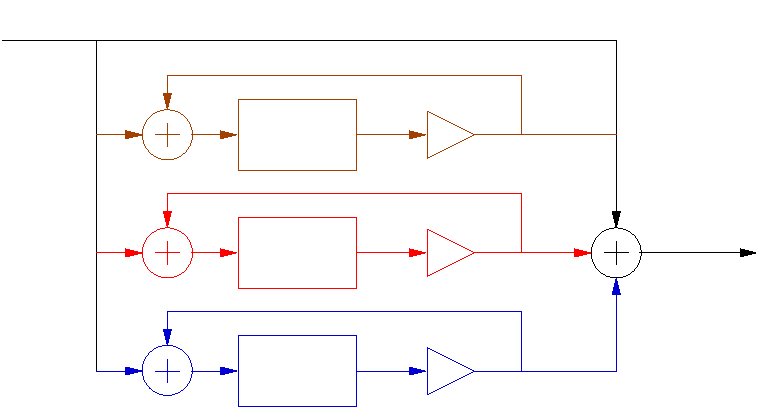
\includegraphics{reverb.pdf}%
\end{picture}%
\setlength{\unitlength}{4144sp}%
%
\begingroup\makeatletter\ifx\SetFigFont\undefined%
\gdef\SetFigFont#1#2#3#4#5{%
  \reset@font\fontsize{#1}{#2pt}%
  \fontfamily{#3}\fontseries{#4}\fontshape{#5}%
  \selectfont}%
\fi\endgroup%
\begin{picture}(5787,3120)(886,-1603)
\put(5493,-512){\makebox(0,0)[lb]{\smash{{\SetFigFont{20}{24.0}{\rmdefault}{\mddefault}{\updefault}{\color[rgb]{0,0,0}$\Sigma$}%
}}}}
\put(2791,1334){}%
\put(901,1334){$x[n]$}%
\put(5896,-286){$y[n]$}%
\put(4321,704){\color[rgb]{.63,.25,0}$g_1$}%
\put(2791,434){\color[rgb]{.63,.25,0}$z^{-d_1}$}%
\put(2791,-466){\color[rgb]{0,0,1}$z^{-d_2}$}%
\put(4321,-241){\color[rgb]{0,0,1}$g_2$}%
\put(4321,-1141){\color[rgb]{1,0,0}$g_3$}%
\put(2791,-1366){\color[rgb]{1,0,0}$z^{-d_3}$}%
\put(2071,389){\makebox(0,0)[lb]{\smash{{\SetFigFont{20}{24.0}{\rmdefault}{\mddefault}{\updefault}{\color[rgb]{.63,.25,0}$\Sigma$}%
}}}}
\put(2071,-512){\makebox(0,0)[lb]{\smash{{\SetFigFont{20}{24.0}{\rmdefault}{\mddefault}{\updefault}{\color[rgb]{0,0,1}$\Sigma$}%
}}}}
\put(2072,-1412){\makebox(0,0)[lb]{\smash{{\SetFigFont{20}{24.0}{\rmdefault}{\mddefault}{\updefault}{\color[rgb]{1,0,0}$\Sigma$}%
}}}}
\end{picture}%
  \caption{The photo shows a block diagram of a \gls{reverb} unit.}
  \label{fig:reverb_block_des}
\end{figure}

From \autoref{fig:reverb_block_des}, the following differential equations can be inferred:

%The equation for the flanger can be written as:
%\begin{equation}
%\label{flang_eq}
%		y[n] = x[n] + x[n- d_{1}] \cdot g_{1}  
%\end{equation}
%
The equation for the delay can be written as:

\begin{equation}
\label{delay_eq}
y[n] = x[n] + \sum_{j=1}^{i}  (x[n- d_{1}] \cdot g_{1})
\end{equation}

%The index $i$ represents the number of delays that are being implemented in the chorus effect which is also the chorus size. Index $n$ represents the number of samples that are being modulated. \\
%If the implementation is done using a time varying delay, equations \ref{flang_eq} and \ref{chor_eq} can be re-written as:
%
%\begin{equation}
%\label{flang_eq2}
%y[n] = x[n] + x[n- d_{1}[n]] \cdot g_{1}  
%\end{equation}
%
%\begin{equation}
%\label{chor_eq2}
%y[n] = x[n] + \sum_{j=1}^{i}  (x[n- d_{j}[n]] \cdot g_{j})
%\end{equation}
%
%The delay value has to be a periodic function that is varying in a user-defined range. 
%
%\subsection{Matlab Simulation}
%
%A delay can be done in different ways digitally. One way is to use a ring buffer also known as circular buffer. \\
%The idea of this data structure is that it takes values and only outputs them when it gets full, and overwrites the oldest after outputting it. It is a kind of a FIFO queue structure but where the start and the overwriting can start at any index. \\
%This means that the size of the buffer depends on the delay.  The buffer size must then be always up-to-date with the new delay value. \\ 
%The value of the delay is determined by a periodic function as said before, different waveforms can be used as said in \autoref{chor_flang}. A common periodic function that can be used is the sine. Since it varies between 0 and 1, it can be then multiplied with the user-defined range. 
%The delay can then be written as:
%
%\begin{equation}
%	d[n]= A \cdot sin(2\pi f_{l} n)
%\end{equation}
%
%$A$ is the value of the user-defined range which is also the depth. $f_{l}$ is the frequency of the LFO. 
%
%The Matlab code for the flanger effect is:
%
%\begin{lstlisting}[language=Matlab, caption= Matlab code for flanger effect]
%
%%Flanger Effect
%%Group 641
%
%%insert your input in this table
%input = [1 2 3 4 5 6 7 8 9 10]
%
%fs = 1;  %LFO Frequency
%sample_no = length(input) %Length of the input
%g = 0.4; %Gain
%after_delay = (1:1:sample_no); 
%before_delay = (1:1:sample_no);
%output = (1:1:sample_no);
%
%for n = 1:1:sample_no
%	delay = 3 * cos((2*pi*fs)/n);  %Calculate time varying delay
%	buffer = zeros(1,abs(round(delay)));
%
%	for i = 1:1:sample_no %loop for an output with one delay value
%		buffer = [buffer(2:end) input(i)];
%		after_delay(i) = buffer(1) * g;
%		before_delay(i) = input(i); 
%		output(i) = after_delay(i) + before_delay(i);
%	end
%	output
%end
%
%plot(output)
%hold on
%grid
%plot(before_delay)
%
%\end{lstlisting}
%
%
%
%
%
